% AI4Research @ ICML 2026 workshop submission.
%
% This file is a self-contained 4-page draft. For final submission, drop the
% body into the official icml2026.sty template (the math, listings, and
% references are template-agnostic). See paper/SUBMISSION-NOTES.md.

\documentclass[10pt,twocolumn,letterpaper]{article}

\usepackage[margin=0.75in]{geometry}
\usepackage{lmodern}

\usepackage{mathtools}
\usepackage{amsthm}
\usepackage{amssymb}
\usepackage{microtype}
\usepackage[hidelinks]{hyperref}
\usepackage{listings}
\usepackage{xcolor}
\usepackage{tikz}
\usetikzlibrary{positioning,arrows.meta,calc}

\setlength{\columnsep}{0.25in}
\setlength{\parskip}{0.2ex}

%% Lean 4 listing style.
\definecolor{leanbg}{rgb}{0.97,0.97,0.97}
\definecolor{leankw}{rgb}{0.10,0.10,0.55}
\definecolor{leanco}{rgb}{0.30,0.50,0.30}
\definecolor{leanst}{rgb}{0.55,0.20,0.20}
\lstdefinelanguage{Lean4}{
  morekeywords={theorem,lemma,def,noncomputable,variable,namespace,end,open,
                section,by,fun,let,in,if,then,else,match,with,do,return,
                instance,class,structure,inductive,where,abbrev,Type,Prop,
                Sort,have,show,exact,intro,intros,apply,refine,calc,using,
                this,rfl,trivial,forall,exists},
  morecomment=[l]{--},
  morecomment=[s]{/-}{-/},
  morestring=[b]",
  sensitive=true,
}
\lstset{
  language=Lean4,
  basicstyle=\ttfamily\scriptsize,
  keywordstyle=\color{leankw}\bfseries,
  commentstyle=\color{leanco}\itshape,
  stringstyle=\color{leanst},
  backgroundcolor=\color{leanbg},
  frame=single,
  framesep=2pt,
  rulecolor=\color{leanbg},
  showstringspaces=false,
  breaklines=true,
  columns=fullflexible,
  keepspaces=true,
  xleftmargin=2pt,
  xrightmargin=2pt,
  aboveskip=4pt,
  belowskip=4pt,
}

%% Math shortcuts.
\newcommand{\Risk}{\mathcal{R}}
\newcommand{\eRisk}{\widehat{\mathcal{R}}}
\newcommand{\KL}{\mathrm{KL}}
\newcommand{\E}{\mathbb{E}}
\newcommand{\R}{\mathbb{R}}
\newcommand{\N}{\mathbb{N}}
\newcommand{\Hyp}{\mathcal{H}}

\title{\vspace{-3ex}\Large\bfseries Machine-Checked PAC-Bayes and Stability Bounds in Lean 4:\\
\large A Finite-First Formalization of Statistical Learning Theory}

\author{Robby Sneiderman \\ \small\texttt{robbysneiderman@gmail.com}}
\date{\vspace{-2ex}}

\begin{document}
\onecolumn
\maketitle
\vspace{-4ex}
\begin{abstract}
\noindent
We present \emph{FormalSLT}, a Lean~4 / Mathlib4 library that delivers
machine-checked proofs of two pillars of statistical learning theory:
the Bousquet--Elisseeff bound on the expected generalization gap of a
uniformly stable algorithm, and a finite-grid McAllester-style PAC-Bayes
confidence bound for $[0,1]$ losses. Both results are stated as Lean
theorems with explicit constants, no asymptotic notation, and no
\texttt{sorry}, \texttt{admit}, or custom axioms. The methodology is
\emph{finite-first}: hypothesis classes are \texttt{Fintype} index types,
samples are product-mass coordinates, and suprema are finite maxima or
supplied boundary functionals. The continuous lift is named as out of scope,
not approximated. The library is 45~modules and 19,339 Lean lines,
complementary to a contemporaneous continuous
empirical-process effort \cite{YuanheZ2026}. Together with the PAC--VC
excess-risk and sample-complexity theorems of \S\ref{sec:library}, these
results give a self-contained finite route from ERM to PAC-Bayes posteriors.
Artifact:
\href{https://github.com/Robby955/lean-statistical-learning}{\nolinkurl{github.com/Robby955/lean-statistical-learning}}.
\end{abstract}
\vspace{1ex}
\twocolumn

\section{Introduction}
\label{sec:intro}

Generalization bounds in machine learning are short on paper and long in
their fine print: every theorem hides a class shape, a boundedness
assumption, a measurability hypothesis, and a constant that rotates each
time the proof is retold. Classical references such as Blumer et~al.\
\cite{Blumer1989} and Bousquet--Elisseeff \cite{BousquetElisseeff2002}
are scrupulous about this; popular textbook presentations
\cite{ShalevShwartz2014, BoucheronLugosiMassart2013} optimize for
readability and trust the reader to reconstruct what is in force at each
step. Errors propagate quietly as the chain lengthens.

This paper contributes \emph{FormalSLT}, a Lean~4 library on top of
Mathlib4 that formalizes a usable slice of statistical learning theory
as a connected chain of machine-checked theorems. The two headline
results we describe here are:
\begin{itemize}\setlength{\itemsep}{0pt}
\item the Bousquet--Elisseeff expected-gap theorem for uniformly stable
  algorithms, in the finite iid product-measure setting; and
\item a finite-grid McAllester-style PAC-Bayes confidence bound for
  $[0,1]$ losses, built on a formalized Donsker--Varadhan variational
  inequality.
\end{itemize}
Every theorem cited compiles against a pinned commit. The full public
spine reduces to the canonical Mathlib axiom set
$\{\texttt{propext},\,\texttt{Classical.choice},\,\texttt{Quot.sound}\}$,
verified by \texttt{\#print axioms} traces in \texttt{examples/}.

The methodology is \emph{finite-first}: hypothesis classes are finite
index types $\iota$ with $[\texttt{Fintype}\;\iota]$, samples are
functions $\texttt{Fin}\,n \to Z$, and the underlying law on $Z$ is a
probability mass function. This scope buys three things at once:
(i)~ML practice already lives there at floating-point resolution;
(ii)~the combinatorial structure of the bounds (Sauer--Shelah growth,
Massart's $\log|\mathcal{H}|$ factor, dyadic chaining) is sharper in
the finite setting; (iii)~the formalization avoids the
$\sigma$-algebra hygiene that dominates continuous empirical-process
arguments. The continuous lift is out of scope and is the natural
composition target for the contemporaneous continuous-empirical-process
effort in Lean~4 \cite{YuanheZ2026}; the missing dependency for each
boundary theorem is named in \texttt{docs/assumptions-and-nonclaims.md}.

\begin{figure*}[!t]
\centering
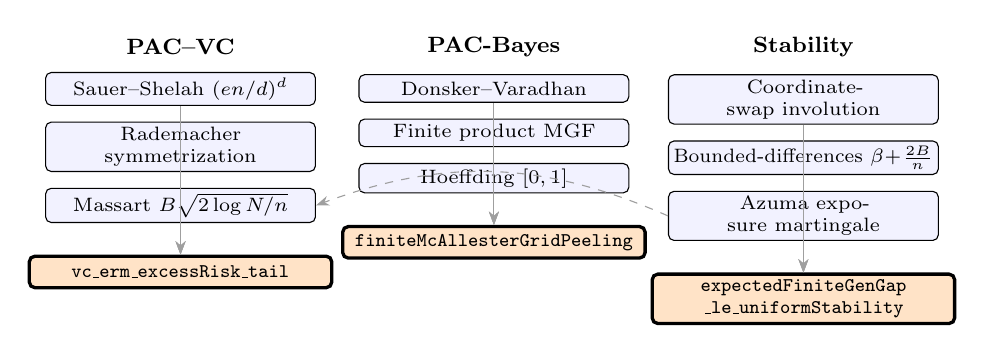
\begin{tikzpicture}[
  node distance=2mm and 4mm,
  every node/.style={font=\scriptsize},
  prim/.style={draw, rounded corners=2pt, fill=blue!5,
               inner sep=1.8pt, align=center, text width=33mm,
               minimum height=3.5mm},
  top/.style={draw, very thick, rounded corners=2pt, fill=orange!22,
              inner sep=2pt, align=center, text width=37mm,
              minimum height=4mm, font=\scriptsize\bfseries},
  hdr/.style={font=\footnotesize\bfseries},
  arr/.style={->, >=Stealth, thin, gray!75}
]
\node[hdr] (hA) {PAC--VC};
\node[hdr, right=22mm of hA] (hB) {PAC-Bayes};
\node[hdr, right=22mm of hB] (hC) {Stability};
\node[prim, below=1mm of hA] (ss)    {Sauer--Shelah $(en/d)^d$};
\node[prim, below=of ss]     (sym)   {Rademacher symmetrization};
\node[prim, below=of sym]    (mass)  {Massart $B\sqrt{2\log N/n}$};
\node[prim, below=1mm of hB] (dv)    {Donsker--Varadhan};
\node[prim, below=of dv]     (mgf)   {Finite product MGF};
\node[prim, below=of mgf]    (hoeff) {Hoeffding $[0,1]$};
\node[prim, below=1mm of hC] (swap)  {Coordinate-swap involution};
\node[prim, below=of swap]   (bd)    {Bounded-differences $\beta+\tfrac{2B}{n}$};
\node[prim, below=of bd]     (azuma) {Azuma exposure martingale};
\node[top, below=4mm of mass]  (vcerm)
  {\texttt{vc\_erm\_excessRisk\_tail}};
\node[top, below=4mm of hoeff] (mca)
  {\texttt{finiteMcAllester\-GridPeeling}};
\node[top, below=4mm of azuma] (stab)
  {\texttt{expectedFiniteGenGap}\\\texttt{\_le\_uniformStability}};
\draw[arr] (ss)    -- (vcerm);
\draw[arr] (sym)   -- (vcerm);
\draw[arr] (mass)  -- (vcerm);
\draw[arr] (dv)    -- (mca);
\draw[arr] (mgf)   -- (mca);
\draw[arr] (hoeff) -- (mca);
\draw[arr] (swap)  -- (stab);
\draw[arr] (bd)    -- (stab);
\draw[arr] (azuma) -- (stab);
\draw[arr, dashed] (azuma.west) to[bend right=22] (mass.east);
\end{tikzpicture}
\caption{Theorem dependency graph. Each blue box is a primitive proved
inside FormalSLT (Mathlib4 supplies the underlying real analysis,
measure theory, Markov, and binomial identities). The three orange
boxes are the named public theorems whose Lean signatures appear in
Listings~\ref{lst:vcerm}, \ref{lst:dv}, \ref{lst:stab}, and
\ref{lst:mca}. The dashed arrow records the cross-track reuse of the
Azuma exposure-martingale tail, which is consumed by both the
generalization-gap step of the PAC--VC route and the
high-probability companion of the stability scaffolding.}
\label{fig:dep}
\end{figure*}

\section{The FormalSLT Library}
\label{sec:library}

\subsection{Architecture}

The 45-module library is organized by spine dependency, summarized in
Figure~\ref{fig:dep}. The PAC--VC core (\texttt{Risk}, \texttt{ERM},
\texttt{Rademacher.*}, \texttt{VC.*}) runs from ERM through symmetrization,
Massart, Sauer--Shelah, and a binary VC bridge to VC ERM excess-risk and
sample-complexity theorems. The PAC-Bayes track
(\texttt{PACBayesKL}, \texttt{PACBayesFiniteProductMGF},
\texttt{PACBayesBoundedLoss}, \texttt{PACBayesMcAllester}) closes finite
Catoni and finite-grid McAllester-style bounds. The stability track
(\texttt{AlgorithmicStability}, \texttt{Stability.BousquetElisseeff}) covers
bounded differences, expected-gap wrappers, and bounded-loss high-probability
surfaces.
A finite-budget Dudley layer (\texttt{Covering.*}), an Azuma-route
exposure-martingale chain (\texttt{Azuma.*}), and a Lipschitz
contraction lemma (\texttt{Rademacher.Contraction}) round out the
spine.

The finite-first methodology is enforced by the Lean type signatures,
not by convention. Every constant is explicit: the high-probability
Rademacher tail is literally $\exp(-\varepsilon^2 n / (8 B^2))$, the
Massart bound is $B\sqrt{2 \log |\Hyp| / n}$, and the Sauer--Shelah
envelope is $(en/d)^d$. There is no $O(\cdot)$ in any theorem
statement.

\subsection{The PAC--VC Spine}

The closing theorem of the PAC--VC track combines the deterministic
ERM inequality, the Sauer--Shelah polynomial bound, Massart's finite-
class bound, and an Azuma-route generalization-gap tail. Its Lean
statement is:

\begin{lstlisting}[caption={VC ERM excess-risk tail
                  (\texttt{FormalSLT/VC/SampleComplexity.lean:334}).},
                  label={lst:vcerm}]
theorem vc_erm_excessRisk_tail
    [MeasurableSpace Z] [StandardBorelSpace Z]
    {mu : Measure Z} [IsProbabilityMeasure mu]
    {l : iota -> Z -> R} {B : R} (hB : 0 < B)
    (hl_meas : forall i, Measurable (l i))
    (hl_bdd  : forall i z, |l i z| <= B)
    {n d : N} (hn : 0 < n) (hd : 0 < d) (hdn : d <= n)
    (hGrowth : ...)  -- effective-class <= sum binomials
    (hhat : (Fin n -> Z) -> iota)
    (hERM : forall S, IsERM (empiricalRisk S l) (hhat S))
    (i_star : iota) {eps : R} (heps : 0 <= eps) :
    (piMeasure mu n).real
        { S | risk mu l i_star
              + 4 * B * Real.sqrt
                  (2 * d * Real.log (Real.exp 1 * n / d) / n)
              + 2 * eps <= risk mu l (hhat S) }
      <= 2 * Real.exp (- eps^2 * n / (8 * B^2))
\end{lstlisting}

\noindent
The user-supplied growth hypothesis is discharged for binary
classifiers under 0/1 loss by a separate \emph{binary VC bridge}
\texttt{effectiveClass\_zeroOneLoss\_card\_le\_sauerShelah}
(\texttt{VC/BinaryVCBridge.lean:154}) that identifies effective loss
patterns with binary class traces. The exponent constant is
$8B^2$ (Azuma route) rather than the textbook $2B^2$ (sharp
McDiarmid); the gap is documented and is awaiting Mathlib's
\texttt{condExpKernel} infrastructure to land.

\subsection{Bousquet--Elisseeff Stability}
\label{sec:stab}

A learning algorithm $A : Z^n \to \iota$ is \emph{uniformly $\beta$-stable}
if replacing one training example shifts the loss of $A(S)$ by at most
$\beta$ on every test point. The library defines this as
\texttt{UniformStability\;A\;l\;beta} and proves the Bousquet--Elisseeff
expected-gap bound in the finite iid product-measure setting:

\begin{lstlisting}[caption={Finite iid Bousquet--Elisseeff expected
                  generalization-gap bound
                  (\texttt{FormalSLT/AlgorithmicStability.lean:1604}).},
                  label={lst:stab},
                  basicstyle=\ttfamily\tiny]
theorem expectedFiniteGeneralizationGap_le_uniformStability_finiteProduct
    {n : N} [Fintype Z] (hn : 0 < n)
    {p : Z -> R} {A : (Fin n -> Z) -> iota}
    {l : iota -> Z -> R} {beta : R}
    (hstab    : UniformStability A l beta)
    (hp_nonneg : forall z, 0 <= p z)
    (hp_sum    : sum z, p z = 1) :
    expectedFiniteGeneralizationGap
        (finiteProductSampleWeight p) p A l <= beta
\end{lstlisting}

\noindent
The proof factors through a finite \emph{coordinate-swap identity} on
the product weight $\prod_k p(S_k)$: replacing the $k$-th sample by an
independent draw is a measure-preserving involution, so swapping
introduces no Jacobian. We pair the expected-gap result with a
high-probability companion: the Bousquet--Elisseeff scaffolding
\texttt{trainingLoss\_hasBoundedDifferences} and
\texttt{stability\_genGap\_hasBoundedDifferences} produce
McDiarmid-style bounded-difference constants $\beta + 2B/n$ and
$2\beta + 2B/n$, which compose with our Azuma-route generalization-gap
tail to deliver a high-probability bound for stable algorithms.

The product-measure lift is also closed under explicit integrability
assumptions, with bounded-loss adapters discharging those assumptions for
finite measurable hypothesis interfaces. The finite version above remains the
clearest statement to audit; the measure-theoretic wrappers provide the
surface used by the bounded-loss Bousquet--Elisseeff high-probability results.

\subsection{PAC-Bayes McAllester at Finite Grid}
\label{sec:pacbayes}

The PAC-Bayes track formalizes the Donsker--Varadhan variational
inequality, the only general change-of-measure ingredient one needs:

\begin{lstlisting}[caption={Donsker--Varadhan variational inequality
                  (\texttt{FormalSLT/PACBayesKL.lean:235}).},
                  label={lst:dv}]
theorem donsker_varadhan [Nonempty iota]
    {rho pi : iota -> R}
    (hrho : IsPMF rho) (hpi : IsFullSupportPMF pi)
    (f    : iota -> R) :
    (sum i, rho i * f i)
      <= klDiv rho pi
       + Real.log (sum i, pi i * Real.exp (f i))
\end{lstlisting}

\noindent
Combined with an exact finite iid product MGF factorization
\texttt{finiteProduct\_mgf\_empiricalRiskDeviation\_eq\_pow} (the
sample-average exponential moment factors as the $n$-th power of the
one-coordinate moment), Hoeffding for $[0,1]$ losses, and Markov's inequality,
this gives a Catoni fixed-$\lambda$ bound plus
\texttt{pac\_bayes\_generalization}: with product-sample mass at least
$1-\delta$, every posterior satisfies the Catoni-form risk bound. A finite
weighted union bound over complexity buckets yields a McAllester-style
square-root bound:

\begin{lstlisting}[caption={Finite-grid McAllester PAC-Bayes confidence
                  bound (\texttt{FormalSLT/PACBayesBoundedLoss.lean:766}).},
                  label={lst:mca}]
theorem finiteMcAllesterGridPeeling_badEventMass_le_delta
    {n : N} [Fintype Z] [Fintype iota] [Fintype gamma]
    [Nonempty iota] (hn : 0 < n)
    (p : Z -> R) (hp : IsPMF p)
    (prior : iota -> R) (hprior : IsFullSupportPMF prior)
    (l : iota -> Z -> R)
    (complexityBound confidenceOf : gamma -> R)
    (hcB    : forall g, 0 < complexityBound g)
    (hcOf   : forall g, 0 < confidenceOf g)
    {delta : R}
    (hgrid  : (sum g, confidenceOf g) <= delta)
    (hl     : forall i z, 0 <= l i z /\ l i z <= 1) :
    (sum S in McAllesterGridPeelingBadSamples ...,
        finiteProductSampleWeight p S) <= delta
\end{lstlisting}

\noindent
Informally: with finite product-sample mass at least $1-\delta$,
\emph{every} posterior $\rho$ in some bucket of the finite complexity
grid satisfies
$\Risk(\rho) \le \eRisk_S(\rho) + \sqrt{C_g/(2n)}$
whenever $\KL(\rho\|\pi) + \log(1/\delta_g) \le C_g$. We make no
claims about all-real-$\lambda$, infinite hypothesis classes, or
continuous posteriors; those are explicit future work and the
non-claims documentation that ships with the library says so.

\section{Related Work}
\label{sec:related}

The closest contemporary effort is YuanheZ et~al.\ \cite{YuanheZ2026},
which formalizes the continuous empirical-process route in Lean~4:
continuous Dudley entropy integrals, Gaussian Lipschitz concentration,
log-Sobolev / Efron--Stein / Poincar\'e functional inequalities,
sparse-regression rates, and minimax lower bounds. Their library and
ours cover disjoint theorem families and are designed to compose: a
reader who needs both directions can use them as joint Lean
dependencies. We do not formalize the continuous Dudley integral or
the functional inequalities; they do not formalize the Sauer--Shelah
polynomial bound, a binary VC bridge, the Bousquet--Elisseeff
expected-gap theorem, or the Donsker--Varadhan / McAllester PAC-Bayes
chain.

A second Lean~4 effort \cite{MohanadAhmed2025} formalizes
symmetrization, Hoeffding, and McDiarmid; the overlap with our spine
is the Rademacher symmetrization step itself. The earliest formalized
PAC learnability theorem is Tassarotti et~al.'s decision-stump proof
in Lean~3 \cite{Tassarotti2021}, whose deterministic / probabilistic
factoring directly informs our split between the finite-sample
sign-vector core and the product-measure envelope. In Coq,
Bagnall--Stewart \cite{BagnallStewart2019} formalize a finite-class
PAC bound via Hoeffding plus a union bound. In Isabelle, Karayel--Tan
\cite{KarayelTan2023} formalize a sharp McDiarmid bound with the
$2B^2$ constant; their development is concentration tooling and does
not connect to PAC, VC, or PAC-Bayes.

\section{Reproducibility and Scope}
\label{sec:scope}

The artifact at
\href{https://github.com/Robby955/lean-statistical-learning}{\nolinkurl{github.com/Robby955/lean-statistical-learning}}
is a Lean~4 / Mathlib4 project. Reproducing the build is two commands:

\begin{lstlisting}[language=]
lake exe cache get
lake build FormalSLT
\end{lstlisting}

\noindent
The audit script greps for executable \texttt{sorry}, \texttt{admit},
and custom \texttt{axiom} or \texttt{constant} declarations within the
\texttt{FormalSLT} and \texttt{examples} directories; the file
\texttt{examples/CheckShowcaseTheorems.lean} carries
\texttt{\#print axioms} traces that pin every public theorem to
$\{\texttt{propext},\,\texttt{Classical.choice},\,\texttt{Quot.sound}\}$.

\paragraph{What is machine-checked.}
The PAC--VC tail and sample-complexity theorem; finite contraction and
linear-predictor bounds; finite Dudley entropy wrappers, truncated-integral
comparisons, and a supplied-supremum adapter; finite and product-measure
Bousquet--Elisseeff expected-gap wrappers; Donsker--Varadhan, finite product
MGF, Catoni, \texttt{pac\_bayes\_generalization}, fixed-budget McAllester, and
finite-grid McAllester peeling.

\paragraph{What is out of scope.}
The continuous Dudley entropy integral; sharp McDiarmid constants
(awaiting Mathlib's \texttt{condExpKernel} API); all-real-$\lambda$,
infinite-hypothesis, and continuous-posterior PAC-Bayes variants;
infinite-class VC theorems. Each boundary is named in
\texttt{docs/assumptions-and-nonclaims.md} with the specific
Mathlib API, Fubini-style lift, or measurability bridge that would
close it.

\paragraph{Reproducibility commitment.}
The release-candidate gate runs three checks: \texttt{lake build
FormalSLT} compiles every cited theorem; an audit script greps for
executable \texttt{sorry}, \texttt{admit}, and custom \texttt{axiom}
declarations and rejects any hit; and
\texttt{examples/CheckShowcaseTheorems.lean} prints the axiom
dependencies of every public theorem in this paper, each pinned to
$\{\texttt{propext},\,\texttt{Classical.choice},\,\texttt{Quot.sound}\}$.
The artifact link in the abstract resolves to a commit-tagged
snapshot.

{\small
\bibliographystyle{plain}
\bibliography{references}
}

\end{document}
